\documentclass[10pt]{beamer}
\usetheme[
%%% option passed to the outer theme
%    progressstyle=fixedCircCnt,   % fixedCircCnt, movingCircCnt (moving is deault)
  ]{Feather}
  
% If you want to change the colors of the various elements in the theme, edit and uncomment the following lines

% Change the bar colors:
%\setbeamercolor{Feather}{fg=red!20,bg=red}

% Change the color of the structural elements:
%\setbeamercolor{structure}{fg=red}

% Change the frame title text color:
%\setbeamercolor{frametitle}{fg=blue}

% Change the normal text color background:
%\setbeamercolor{normal text}{fg=black,bg=gray!10}

%-------------------------------------------------------
% INCLUDE PACKAGES
%-------------------------------------------------------

\usepackage[utf8]{inputenc}
\usepackage[english]{babel}
\usepackage[T1]{fontenc}
\usepackage{helvet}

%-------------------------------------------------------
% DEFFINING AND REDEFINING COMMANDS
%-------------------------------------------------------

% colored hyperlinks
\newcommand{\chref}[2]{
  \href{#1}{{\usebeamercolor[bg]{Feather}#2}}
}

%-------------------------------------------------------
% INFORMATION IN THE TITLE PAGE
%-------------------------------------------------------

\title[] % [] is optional - is placed on the bottom of the sidebar on every slide
{ % is placed on the title page
      \textbf{Docker 101}
}

\subtitle[Docker hands-on]
{
      \textbf{A very basic hands-on introduction}
}

\author[Allan Costa]
{      Allan Costa\\
	  {\ttfamily @allanino}
}

\date{\today}

%-------------------------------------------------------
% THE BODY OF THE PRESENTATION
%-------------------------------------------------------

\begin{document}

%-------------------------------------------------------
% THE TITLEPAGE
%-------------------------------------------------------

{\1% % this is the name of the PDF file for the background
\begin{frame}[plain,noframenumbering] % the plain option removes the header from the title page, noframenumbering removes the numbering of this frame only
  \titlepage % call the title page information from above
\end{frame}}

%-------------------------------------------------------
\begin{frame}{About the author}
%-------------------------------------------------------
	%An unusual background:
	%\begin{itemize}
	%	\item Mathematics at Uni-FACEF, Franca-SP. Finished!
	%	\item Astronomy at USP, São Paulo-SP. Quit after three semesters.
	%	\item Physics at USP, São Paulo-SP. Quit after one semester.
	%	\item System Analysis at Fatec, Franca-SP. Quit after four semesters.
	%	\item Masters in Mathematics at UFSCar, São Carlos-SP. Finishing \textbackslash %o/
	%\end{itemize}
	
	Started to work as developer at CloudWalk in August, 2013, having as goal to research and apply Machine Learning techniques to our business.

	\begin{figure}[h!]
		\centering
		
\includegraphics[width=0.7\textwidth]{images/cloudwalk-logo.png}
	\end{figure}
	
	Docker was launched as an open-source project in March, 2013, so I didn't get a chance to live in dependency hell.
	
	\vspace{0.5cm}
	
	Some of my personal projects: \url{http://allanino.me/projects}
\end{frame}

%-------------------------------------------------------
\begin{frame}{Content}{}
%-------------------------------------------------------
	\vspace{0.15cm} % Needed this to fix a quite large table of contents
	\tableofcontents
\end{frame}

%-------------------------------------------------------
%-------------------------------------------------------
\section{What is Docker?}
%-------------------------------------------------------
\subsection{It's not a VM}
\begin{frame}{What is Docker?}{It's not a VM!}
%-------------------------------------------------------
	\begin{figure}[h!]
		\centering
		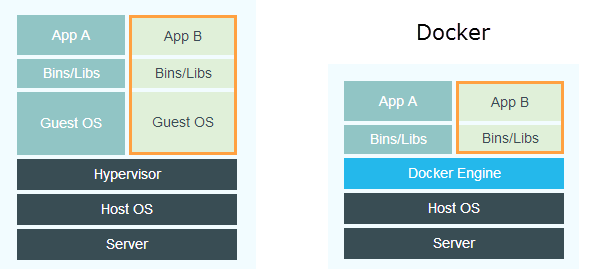
\includegraphics[width=0.9\textwidth]{images/vm-vs-docker.png}
	\end{figure}
	
	\vspace{1cm}
	\scriptsize{\textit{Source:} \url{http://www.jayway.com/2015/03/21/a-not-very-short-introduction-to-docker/}}
\end{frame}
%-------------------------------------------------------
\subsection{It's more than Docker Engine}
\begin{frame}{What is Docker?}{It's more than Docker Engine}
%-------------------------------------------------------
	\begin{figure}[h!]
		\centering
		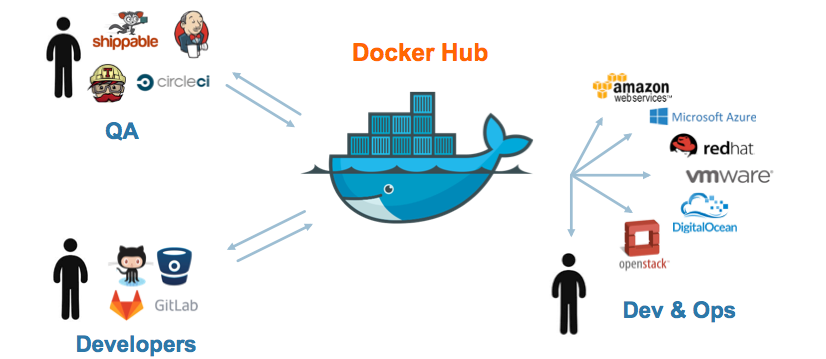
\includegraphics[width=1.\textwidth]{images/docker-hub-diagram.png}
	\end{figure}
	
	\vspace{1.2cm}
	\scriptsize{\textit{Source:} \url{https://blog.docker.com/2015/09/docker-hub-2-0/}}
\end{frame}
%-------------------------------------------------------
\subsection{It's a whole ecosystem}
\begin{frame}{What is Docker?}{It's a whole ecosytem}
%-------------------------------------------------------
	\begin{figure}[h!]
		\centering
		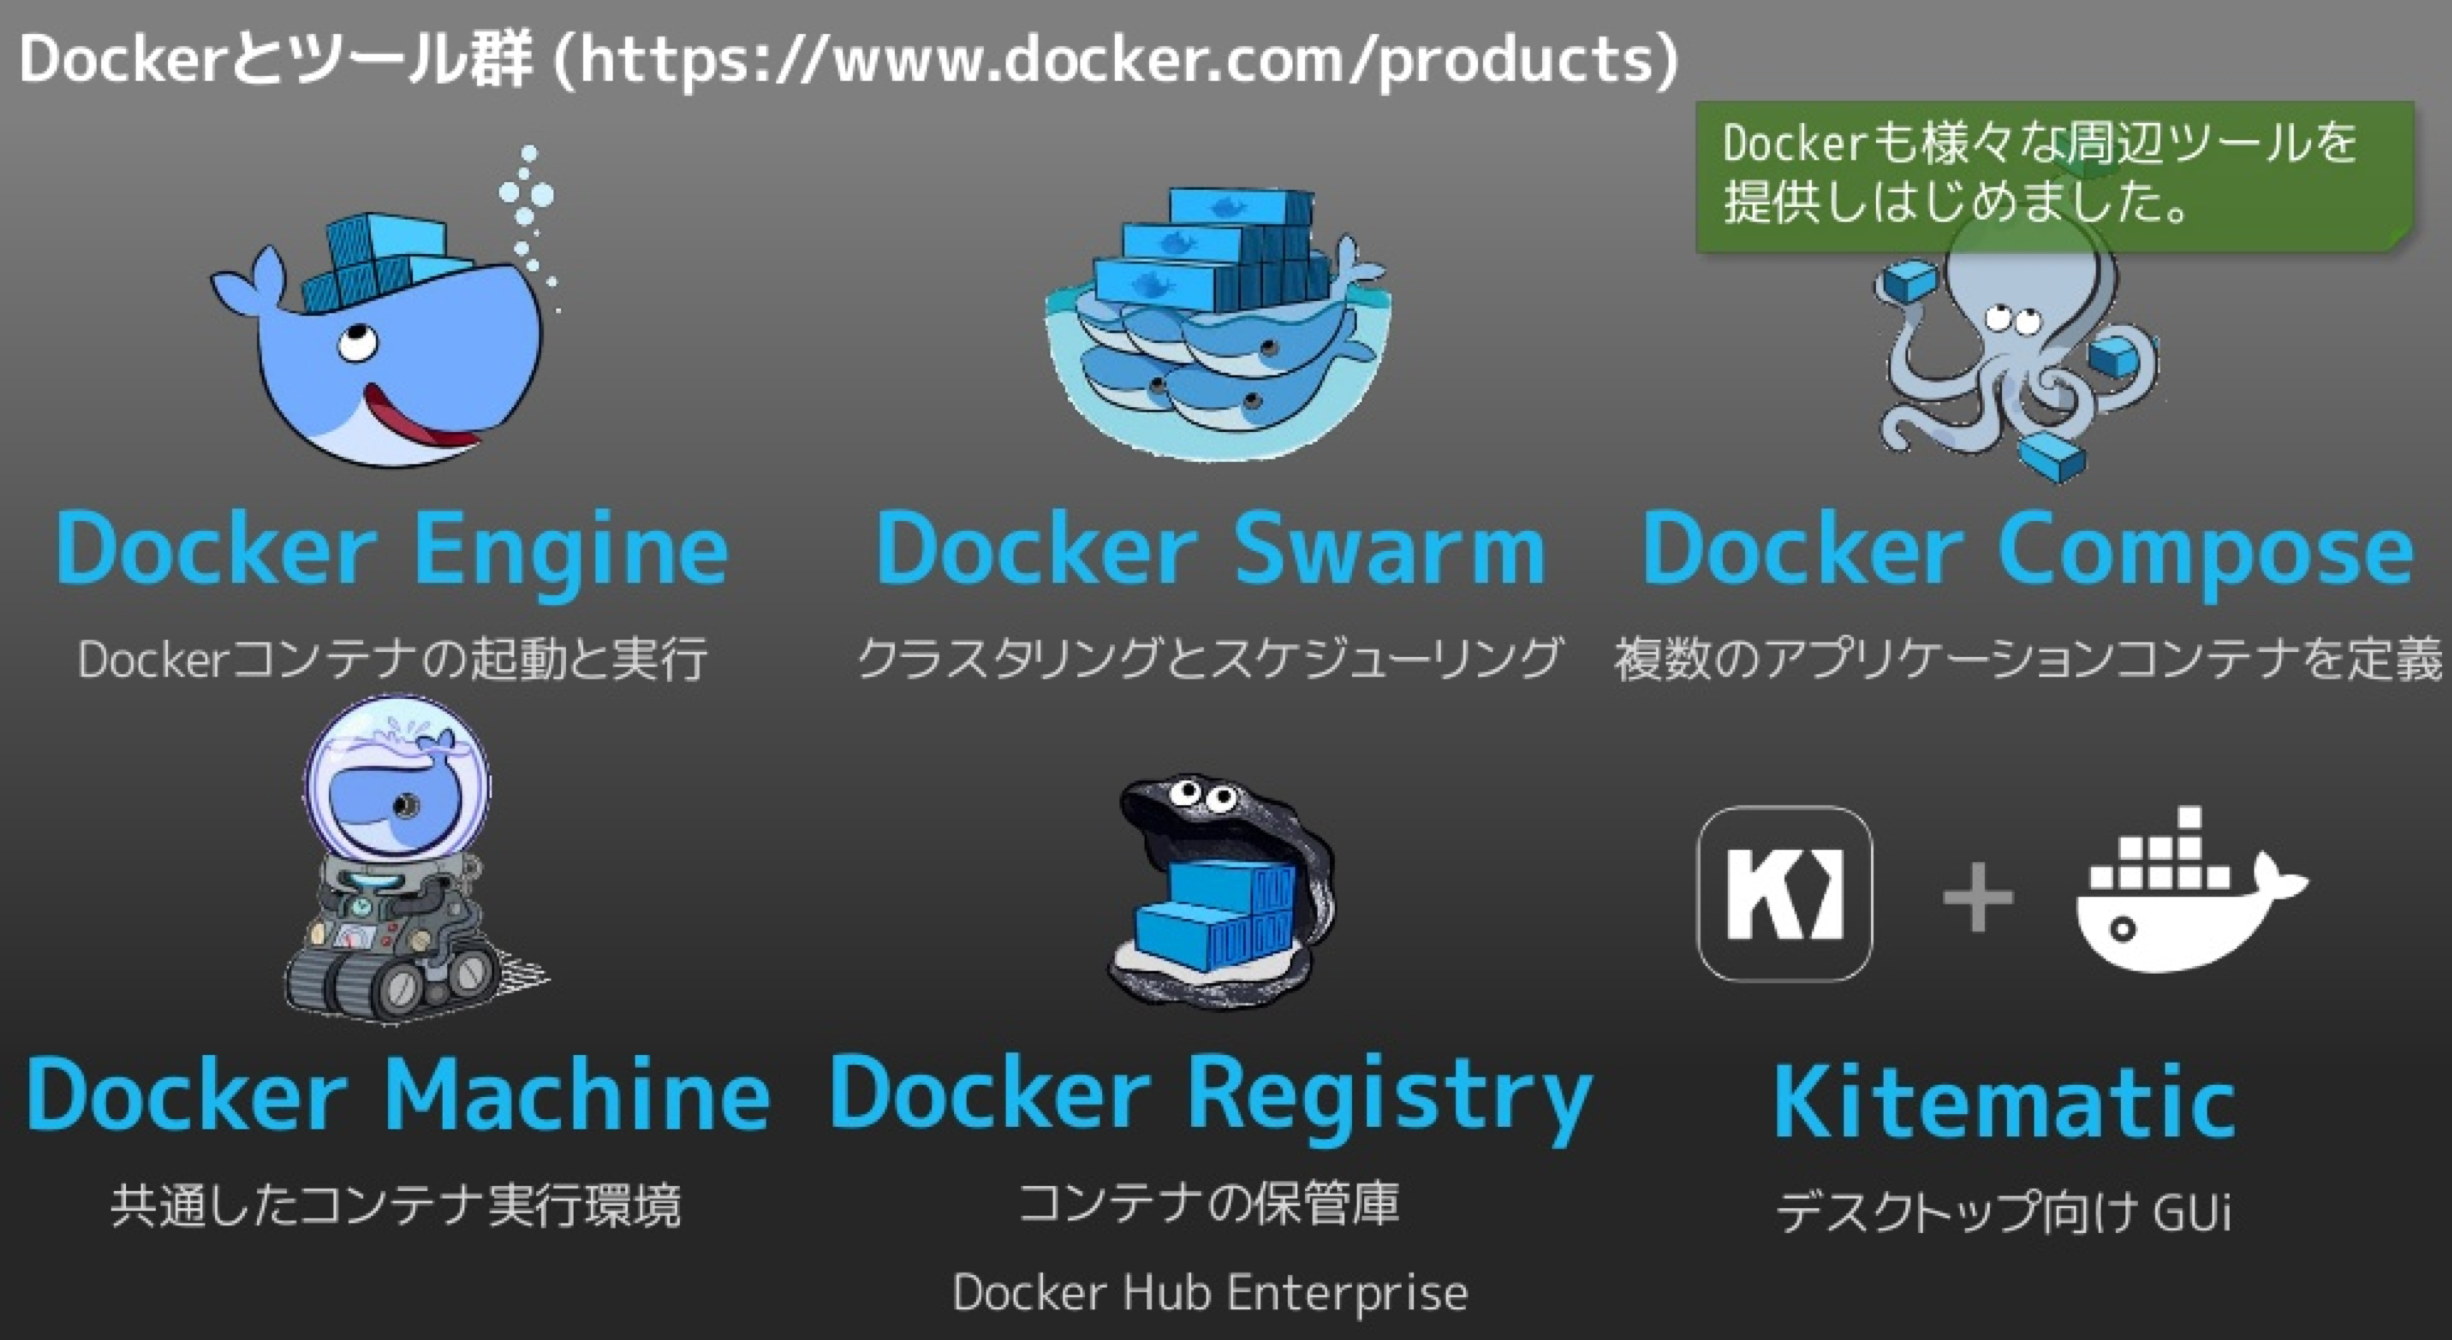
\includegraphics[width=1.\textwidth]{images/docker-ecosystem.png}
	\end{figure}
	
	\vspace{0.1cm}
	\scriptsize{\textit{Source:} \url{https://gist.github.com/j138/9db77cd23133b72dfbc1}}
\end{frame}

%-------------------------------------------------------
%-------------------------------------------------------
\section{Installation}
%-------------------------------------------------------
\begin{frame}{Installation}
%-------------------------------------------------------
	We need for this tutorial to install Docker Engine and Docker Compose. It's really platform specific, so please refer to the docs:
	
	\begin{center}
		\url{https://docs.docker.com/engine/installation/} \\
		\url{https://docs.docker.com/compose/install/}
	\end{center}
	
	Non-Linux users should try installing Docker Toolbox, which contains the tools we need plus a nice GUI (Kitematic) and Docker Machine:
	
	\begin{center}
		\url{https://www.docker.com/products/docker-toolbox}
	\end{center}
\end{frame}

%-------------------------------------------------------
%-------------------------------------------------------
\section{Docker images}
%-------------------------------------------------------
\subsection{Using a Dockerfile to build an image}
\begin{frame}[fragile]{Docker images}{Using a Dockerfile to build an image}
%-------------------------------------------------------
	First, let's clone this presentation's repository in GitHub. It contains our example
	source code:
	\begin{verbatim}
	$ git clone git@github.com:allanino/docker-presentation.git
	$ cd docker-presentation
	\end{verbatim}
	
	Take a look at our project's \texttt{Dockerfile}:
	\begin{verbatim}
	$ cat Dockerfile
	FROM gliderlabs/alpine:3.2
	MAINTAINER Allan Costa "allaninocencio@yahoo.com.br"
	RUN apk --update add python-dev py-pip
	ADD . /src/app
	WORKDIR /src/app
	RUN pip install -r requirements.txt
	ENTRYPOINT ["python", "app.py"]
	\end{verbatim}
	
	Use our Dockerfile to build a Docker image:
	\begin{verbatim}
		$ docker build -t allanino/app .
	\end{verbatim}
\end{frame}
%-------------------------------------------------------
\subsection{Running a container}
\begin{frame}[fragile]{Docker images}{Running a container}
%-------------------------------------------------------
	To start a container from our image we just need to run this command:
	\begin{verbatim}
	$ docker run -p 80:5000 allanino/app
	\end{verbatim}
	
	The only parameter we passed, using the \texttt{-p} flag, was to map container's port 5000 to host's port 80. In this way, the application should be available on \url{http://localhost}.
	
	\vspace{0.5cm}
	WARNING: Don't try to access \url{http://localhost/counter}.
\end{frame}
%-------------------------------------------------------
\subsection{Pushing the image to Docker Hub}
\begin{frame}[fragile]{Docker images}{Pushing the image to Docker Hub}
%-------------------------------------------------------
	We can manually push an image to a registry, but before doing that, you need to login to your account, in this case a Docker Hub account:
	
	\begin{verbatim}
	$ docker login
	\end{verbatim}

	Then push the image to a repository with same name:
	\begin{verbatim}
	$ docker push allanino/app
	\end{verbatim}
	
	
	After the image is uploaded, anyone can pull it (if it's public) using this command:
	\begin{verbatim}
	$ docker pull allanino/app
	\end{verbatim}
\end{frame}

%-------------------------------------------------------
%-------------------------------------------------------
\section{Continuous integration}
%-------------------------------------------------------
\subsection{Automate build}
\begin{frame}{Continuous integration}{Automate build}
%-------------------------------------------------------
	We can integrate source control platforms, such as GitHub or Bitbucket, to have images built automatically on code change.
	
	\vspace{0.5cm}
		
	One platform we use, specially for automatic image tagging based on Git tags, is \url{quay.io}:
	\begin{figure}[h!]
		\centering
		
\includegraphics[width=.75\textwidth]{images/quay_preview.png}
	\end{figure}
\end{frame}

%-------------------------------------------------------
%-------------------------------------------------------
\section{Orchestration}
%-------------------------------------------------------
\subsection{Why we need it}
\begin{frame}{Orchestration}{Why we need it}
%-------------------------------------------------------
	\begin{center}
		Monolithic servers x Microservices
	\end{center}
\end{frame}
%-------------------------------------------------------
\subsection{A multi-container application}
\begin{frame}[fragile]{Orchestration}{A multi-container application}
%-------------------------------------------------------
	What about adding a Redis database?

	\begin{verbatim}
	$ docker run --name redis redis
	\end{verbatim}

	Let's give our application access to it:

	\begin{verbatim}
	$ docker run --name app --link redis:db -p 80:5000 \
    allanino/app
	\end{verbatim}

	Check container's environment variables:
	\begin{verbatim}
	$ docker exec app env
	\end{verbatim}
\end{frame}
%-------------------------------------------------------
\subsection{Docker Compose: creating a configuration file}
\begin{frame}[fragile]{Orchestration}{Docker Compose: creating a configuration file}
%-------------------------------------------------------
	Create a \texttt{docker-compose.yml} file:
	\begin{verbatim}
version: '2'
services:
  app:
    build: .
    ports:
      - "80:5000"
    volumes:
      - .:/src/app
    links:
      - redis
  redis:
    image: redis
      volumes:
        - redis_data:/data
volumes:
  redis_data:
    driver: local
	\end{verbatim}
\end{frame}
%-------------------------------------------------------
\subsection{Docker Compose: running the project}
\begin{frame}[fragile]{Orchestration}{Docker Compose: running the project}
%-------------------------------------------------------
	With Compose we can start our entire project with a single command:
	
	\begin{verbatim}
	$ docker-compose up
	\end{verbatim}
	
	You can scale individual services when running a swarm:
	\begin{verbatim}
	$ docker-compose scale app=3
	\end{verbatim}
	
	Obs: The command above will probably fail for you, because you are probably not running a swarm. 
\end{frame}

%-------------------------------------------------------
%-------------------------------------------------------
\section{What's next}
%-------------------------------------------------------
\begin{frame}{What's next}
%-------------------------------------------------------
	\begin{itemize}
		\item \textbf{Docker Machine:} provision and manage multiple remote Docker hosts.
		\item \textbf{Docker Swarm:}  turns a pool of Docker hosts into a single, virtual Docker host.
	\end{itemize}
\end{frame}
	
{\1
\begin{frame}[plain,noframenumbering]
  \finalpage{{\LARGE Thank you!}}
\end{frame}}

\end{document}